\documentclass[border=8pt]{standalone}
\usepackage[T1]{fontenc}
\usepackage{tgpagella}
\usepackage{tikz}
\usetikzlibrary{arrows.meta,positioning,fit,backgrounds}

\definecolor{ink}{HTML}{16140F}
\definecolor{mid}{HTML}{5C5849}
\definecolor{navy}{HTML}{2E5B88}
\definecolor{navybg}{HTML}{EBF1F6}
\definecolor{ochre}{HTML}{B86B28}
\definecolor{ochrebg}{HTML}{FAF2EA}
\definecolor{paper}{HTML}{F7F5EE}

\tikzset{
  blk/.style={draw=ink,line width=0.6pt,rounded corners=2pt,fill=white,font=\small,align=center,inner sep=5pt},
  blkg/.style={blk,fill=paper},
  blkn/.style={blk,fill=navy!18},
  blko/.style={blk,fill=ochre!22},
  arr/.style={-{Stealth[length=2.2mm]},line width=0.6pt,draw=ink},
  darr/.style={arr,dashed},
  grp/.style={draw=mid,dashed,line width=0.5pt,rounded corners=3pt,inner sep=7pt},
  lbl/.style={font=\scriptsize\itshape,text=mid},
}

\begin{document}
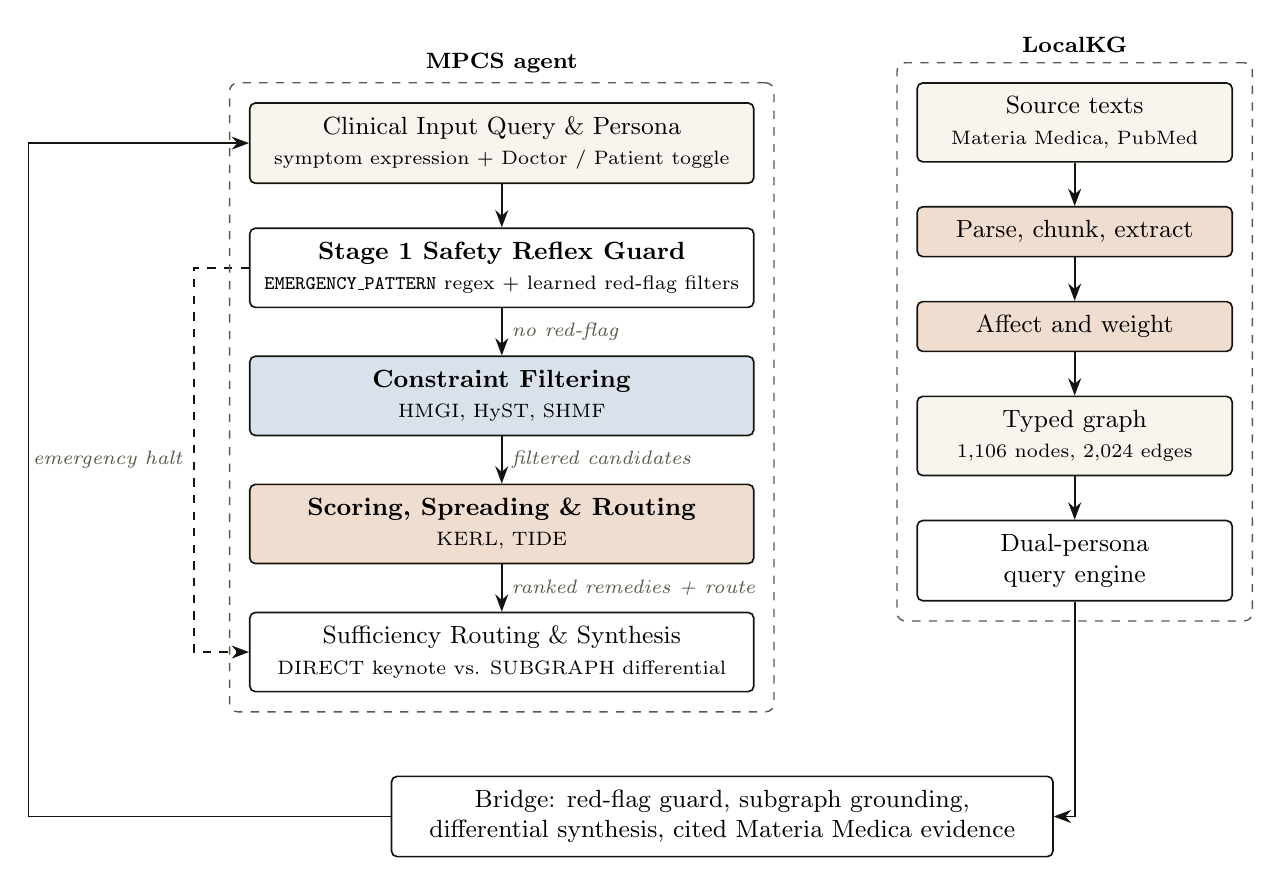
\begin{tikzpicture}[node distance=5.5mm and 8mm]
  % MPCS column
  \node[blkg,minimum width=64mm] (perc) {Clinical Input Query \& Persona\\\scriptsize symptom expression + Doctor / Patient toggle};
  \node[blk,below=of perc,minimum width=64mm] (refl) {\textbf{Stage 1 Safety Reflex Guard}\\\scriptsize \texttt{EMERGENCY\_PATTERN} regex + learned red-flag filters};

  % Retrieval & TIDE deliberation
  \node[blkn,below=6mm of refl,minimum width=64mm] (ret_blue) {\textbf{Constraint Filtering}\\\scriptsize HMGI, HyST, SHMF};
  \node[blko,below=6mm of ret_blue,minimum width=64mm] (ret_brown) {\textbf{Scoring, Spreading \& Routing}\\\scriptsize KERL, TIDE};

  \node[blk,below=6mm of ret_brown,minimum width=64mm] (dec) {Sufficiency Routing \& Synthesis\\\scriptsize DIRECT keynote vs. SUBGRAPH differential};

  \draw[arr] (perc) -- (refl);
  \draw[arr] (refl) -- node[lbl,right]{no red-flag} (ret_blue);
  \draw[arr] (ret_blue) -- node[lbl,right]{filtered candidates} (ret_brown);
  \draw[arr] (ret_brown) -- node[lbl,right]{ranked remedies + route} (dec);
  \draw[darr] (refl.west) -- ++(-7mm,0) |- node[lbl,pos=0.25,left=3pt,fill=white,inner sep=1pt]{emergency halt} (dec.west);

  \node[grp,fit=(perc)(refl)(ret_blue)(ret_brown)(dec),label={[font=\footnotesize\bfseries]above:MPCS agent}] (g1) {};

  % LocalKG column
  \node[blkg,right=18mm of g1.north east,anchor=north west,minimum width=40mm] (src) {Source texts\\\scriptsize Materia Medica, PubMed};
  \node[blko,below=of src,minimum width=40mm] (ext) {Parse, chunk, extract};
  \node[blko,below=of ext,minimum width=40mm] (aff) {Affect and weight};
  \node[blkg,below=of aff,minimum width=40mm] (kg) {Typed graph\\\scriptsize 1,106 nodes, 2,024 edges};
  \node[blk,below=of kg,minimum width=40mm] (qe) {Dual-persona\\query engine};
  \draw[arr] (src)--(ext); \draw[arr] (ext)--(aff); \draw[arr] (aff)--(kg); \draw[arr] (kg)--(qe);
  \node[grp,fit=(src)(ext)(aff)(kg)(qe),label={[font=\footnotesize\bfseries]above:LocalKG}] (g2) {};

  % Bridge
  \node[blk,below=8mm of g1.south,xshift=28mm,minimum width=84mm] (br) {Bridge: red-flag guard, subgraph grounding,\\differential synthesis, cited Materia Medica evidence};
  \draw[arr] (qe.south) |- (br.east);
  \draw[arr] (br.west) -| ([xshift=-28mm]perc.west) -- (perc.west);
\end{tikzpicture}
\end{document}
